\documentclass{article}
\setlength\parindent{0pt}
\usepackage[hmargin=2.5cm,vmargin=2.5cm,bindingoffset=0.5cm]{geometry}
\usepackage{graphicx}
\usepackage{mathtools}
\usepackage{amsthm}
% \usepackage{amsmath}
\usepackage{amsfonts}
\usepackage{changepage}
\newcommand{\norm}[2]{\left \lVert #1 \right \rVert_{#2}}
\setlength{\abovecaptionskip}{-0pt}
\newtheorem{theorem}{Theorem}
\graphicspath{{../images}{}}
\begin{document}\begin{center}
\LARGE \textsc{The $k$-Means Clustering Algorithm}\\
\Large \textsc{Mth 445}\\
\large Russell Breaux\\
%\hrulefill
\begin{figure}[h!]
 \centering
  \vspace{-0.5cm}
  
\includegraphics[width=1.0\textwidth]{normal_nobackground1.png}
  \vspace{-1.0cm}
 \end{figure}
\end{center}
\begin{section} {Gaussian Mixture Models}
\textbf{Multidimensional Gaussian models:} We characterize the Gaussian distribution of some $n$-dimensional vector $X$ by 
\[X \sim  \mathcal{N}(\mu,\Sigma),\]
where  $\mu$ and $\Sigma$ denote the mean and covariance matrix of $X$, respectively. Note that the covariance matrix of a real random vector must be postive semi-definite. If in addition the covariance matrix of $X$ is invertible, $X$ has a density given by 
\[f(x) = \frac{1}{\sqrt{(2\pi)^{n}\lvert\Sigma\rvert}}e^{-\frac{1}{2}(x-\mu)^T\Sigma^{-1}(x-\mu)}\]
where $\lvert\Sigma\rvert$ is the determinant of the covariance matrix.\\

\textbf{Gaussian mixture models:} Suppose we have $k$ such distributions $f_1,\ldots,f_k$ beholden to parameters $(\mu_1,\Sigma_1),\ldots,(\mu_k,\Sigma_k)$, respectively. Let $\pi_1,\ldots,\pi_k$ be any probability distributions on $\{1,\ldots,k\}$. Consider the $j$-th distribution with probability $\pi_j$. We have
\[X \sim \mathcal{N}(\mu_Z,\Sigma_Z)\quad\text{with}\quad Z\sim\pi\]
The vector $X$ has density given by
\begin{equation}
p_\theta(x) = \sum_{j=1}^{k}{\pi_jf_j(x)},
\end{equation}
where the parameter $\theta = (\mu, \pi, \Sigma)$ consists of:
\begin{itemize}
	\item the mixing distribution $\pi = (\pi_1,\ldots,\pi_k)$,
	\item the set of means  $\mu = (\mu_1,\ldots,\mu_k)$,
	\item the set of covariance matrices $\Sigma = (\Sigma_1,\ldots,\Sigma_k)$.
\end{itemize}
\textbf{Maximizing likelihood:} Suppose we wish to estimate the parameter $\theta$ based on $n$ i.i.d. samples $x_1,\ldots,x_n$ taken from the Gaussian mixture model. Let $x$ denote the vector $(x_1,\ldots,x_n)$. The likelihood of $x$ is given by
\begin{equation}
p_\theta(x) = \prod_{i=1}^{n}{p_\theta(x_i)},
\end{equation}
and the log-likelihood by
\[\ell(\theta) = \log{p_{\theta(x)}} = \sum_{i=1}^{n}{\log{p_{\theta(x_i)}}}.\]
By (1), we have
\[\ell(\theta) = \sum_{i=1}^{n}{\log{\left(\sum_{j=1}^{k}{\pi_{j}f_{j}(x_i)}\right)}}.\]
Thus the maximum likelihood estimator of $\theta$ is
\[\theta^{*} = \arg\max_{\theta}{\ell(\theta)}.\]
\end{section}
\begin{section}{Clustering Algorithms}
\textbf{Clustering:} Given a set of $N$ vectors $\{x_{1},\ldots,x_{N}\}\subset\mathbb{R}^{n}$,  a \textit{clustering} of the set seeks to partition the vectors into $k$ groups or \textit{clusters} such that distances between pairs of vectors in the same cluster are minimized. Clustering is widely used for various data science and machine learning tasks,  usually when the discrete elements of each vector represent individual characteristics, or \textit{features}, of an object. A \textit{clustering algorithm} defines a particular formula for assigning vectors to a cluster, called the \textit{update formula}, as well as a metric for measuring the relative tightness of a cluster partition,  called the \textit{objective function.} Clustering algorithms run by iteratively applying the update formula to the dataset and using the objective function to measure the improvement in intra-cluster distance minimization.  Typically $N$ is much larger than $k$, with most common applications using values of $k$ ranging from single-digits to values in the hundreds, and values of $N$ ranging from hundreds to billions or more.  Figure 1 shows a simple example of a $k=3$ clustering in $n=2$ dimesions. Such well defined clusters are rare in real-world applications, and the number of features is typically  much higher than 2. 

\begin{figure}[h!]
 \centering
  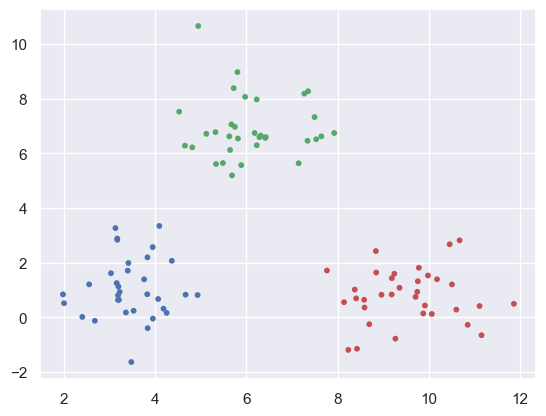
\includegraphics[width=0.5\textwidth]{example_cluster.png}
 \caption{A clustering with $n$ = 2 features and $k=3$ clusters}
 \end{figure}

\textbf{Cluster assignments:} To specify a particular clustering of the set of vectors, we begin by labeling the clusters with the integers $\{1,\ldots,k\}$. We then store the cluster assignments of each data vector in an $N$-vector $c$, where $c_{i}$ stores the label of the group to which $x_{i}$ has been assigned. For example, imagine we partition a dataset with $N=7$ vectors into $k=3$ groups, and suppose we have $c=(3,1,2,2,2,3,1)$. This cluster assignment vector places $x_{1}$ and $x_{6}$ into group 3, $x_{2}$ and $x_{7}$ into group 1, and $x_{3}$, $x_{4}$, and $x_{5}$ into group 2. We also describe the clustering assignments using the sets of indices of vectors belonging to each group. Let $G_{j}$ be the set of indices corresponding to cluster $j$. Then for the above example, we have
\[G_{1} = \{2,7\},\qquad G_{2} = \{3,4,5\},\qquad G_{3} = \{1,6\}.\]
Formally, we have 
\[G_{j}\,\dot{=}\,\{i \mid c_{i} = j\},\]
which defines group $G_{j}$ as the set of all indices $i$ for which $c_{i} = j$.\\

\textbf{Group representatives:} For each cluster we calculate a \textit{group representative} $n$-vector, denoted by $\{z_{1},\ldots ,z_{k}\}$. These vectors are synthesized from information about our clusters, and are not members of the dataset. Our distance minimization goal leads us to seek a value of each $z_{j}$ such that
\[\norm{x_{i} - z_{c_{i}}}{2}\]
is small. Here, $c_{i}$ denotes the group to which $x_{i}$ belongs, so $z_{c_{i}}$ is the group representative of that group. We will soon show that the best choice of $z_j$ is $\mu_j$, the mean of all vectors in group $j$. Note that our measure of distance is the Euclidean 2-norm.\\

\textbf{The objective function:} The standard variant of the $k$-means algorithm uses the within-cluster sum of squares (WCSS) divided by the number of elements, given by
\begin{equation}
J^{\text{clust}}=\left(\norm{x_{1} - z_{c_{1}}}{2}^{2}+\cdots+\norm{x_{N} - z_{c_{N}}}{2}^{2}\right)/N,
\end{equation}
which measures the mean-square distance from the data vectors to their respective representatives. Note that $J^{\text{clust}}$ is the sum of the variances of each cluster, where the group representatives $z_{1},\ldots,z_{k}$ are chosen for $\mu_1,\ldots,\mu_k$. We see that the value of $J^{\text{clust}}$ is impacted both by the cluster assignments of each data vector as well as the choice of representative for each group. This makes perfect sense given our goal of minimizing within-group distances, but note that other objective functions are often used, particularly for data that form non-spherical clusters.
\end{section}
\begin{section}{The $\boldmath{k}$-Means Algorithm}
\textbf{Derivation from Gaussian mixtures:} We now consider a special and simple case of the Gaussian mixture model. Consider such a model with diagonal covariance matrix $\sigma^2I$ for some parameter $\sigma > 0$, and uniform mixing distribution given by
\[X \sim \mathcal{N}(\mu_Z,\sigma^2I)\quad\text{with}\quad Z \sim \mathcal{U}(\{1,\ldots,k\}).\]
The density of $X$ simplifies considerably to
\[f(x) = \frac{1}{k}\sum_{j=1}^{k}{f_j(x)},\]
with
\[f_j(x) = \frac{1}{(2\pi\sigma^2)^{\frac{n}{2}}}e^{\frac{-\norm{x-\mu_j}{2}^{2}}{2\sigma^{2}}}.\]
If we assume the variance $\sigma^{2}$ is known, our only remaining a parameter is $\theta = \mu$, the vector of means which we've denoted by $z_1,\ldots,z_k$. With this assumption we have the $k$-means model.\\

\textbf{The algorithm:} We have established two ways by which a clustering can be improved: by reassigning data vectors to the cluster with the nearest representative, and by recalculating the representatives to better fit their respective clusters.  While performing these tasks simultaneously would ensure the discovery of the \textit{optimal} solution---the global minimum value of $J^{\text{clust}}$---the computational complexity of this task grows staggeringly fast with the value of $N$. Instead, the $k$-means algorithm performs these tasks iteratively to find a solution that, while potentially \textit{suboptimal}, yields a value of $J^{\text{clust}}$ that is typically quite close to its optimal value. We summarize the steps of a single iteration below.\\

\adjustwidth{3em}{0pt}\textbf{1. Partition the data vectors:} Fix $\{z_1,\ldots ,z_k\}$. For the first iteration, it is typical to randomly generate the group representatives within the bounds of the dataset, but certain techniques like principal component analysis can yield better initial representatives. After generating the initial representatives, we seek optimal values for the group assignments $c_1,\ldots ,c_N$ such that $J^{\text{clust}}$ is minimized. Encouragingly, the optimal minimization can be found with certainty for a fixed set of group representatives. Recall that $J^{\text{clust}}$ is a sum of $N$ terms, and that each choice of $c_i$ affects only the $i^{th}$ term of $J^{\text{clust}}$ given by $(1/N)\norm{x_{i} - z_{c_{i}}}{2}^{2}$. Hence choosing each $c_i$ independently such that $\norm{x_{i} - z_{c_{i}}}{2}$ is minimized will yield an optimal minimum value of $J^{\text{clust}}$ for our fixed representatives. Choosing the group assignments in this way gives
\[\norm{x_{i} - z_{c_{i}}}{2} = \min_{j \in \{1,\ldots,k\}}\norm{x_{i} - z_{j}}{2}\]
with a resulting $J^{\text{clust}}$ value given by
\[J^{\text{clust}} =  \left(\min_{j \in \{1,\ldots,k\}}\norm{x_{1} - z_{j}}{2}^{2}+\cdots+\min_{j \in \{1,\ldots,k\}}\norm{x_{N} - z_{j}}{2}^{2}\right )/N\]

\textbf{2. Calculate group representatives:} Now that we have determined the optimal cluster assignments given our current representatives, we fix the cluster assignments of the data vectors and recalculate the group representatives to be the centroids of each cluster.  Fortunately, this step also yields an optimal solution given a fixed clustering. To find the values of $z_1,\ldots,z_k$ that minimize $J^{\text{clust}}$, it is helpful to break our objective function into summands that represent the contribution of each cluster to the total value of $J^{\text{clust}}$. Define $J_1,\ldots,J_k$ to be the contributions of each cluster to the value of $J^{\text{clust}}$, and recall that $G_j$ denotes the set of indices $i$ for which $x_i$ is assigned to cluster $j$. We have,
\[J^{\text{clust}} = \sum_{i=1}^{k}{J_i}\:,\]
where $J_j$ is given by
\[J_j = \frac{1}{N}\sum_{i \in G_j}{\norm{x_i - z_j}{2}^{2}}\]

Thus we seek a value of $z_j$ that minimizes the mean squared distance from $z_j$ to the vectors in cluster $j$. Choosing $z_j$ as the centroid for each group will minimize this value, so defining $z_j$ in this manner gives
\[z_j = \frac{1}{|G_j|}\sum_{i\in{G_j}}{x_i} \tag{2}\]  

To show that this value of $z_j$ does in fact minimize the objective function, we provide a statement of the claim and a brief proof.\\
\begin{theorem}
The centroid of a set of vectors optimally minimizes the mean of squared distances to the vectors in the set.
\end{theorem}
\begin{proof}
Let $J(z)$ denote the mean squared distance from a vector $z$ to the $m$ elements in some set of vectors $G$.  Let $\overline{x} = (x_1+\cdots+x_m)/m$ denote the mean of these elements. We have
\begin{align*}
J(z) &= \frac{1}{m}\sum_{i = 1}^{m}{\norm{x_i - z}{2}^{2}}
\shortintertext{Rewriting in terms of $\overline{x}$,}
J(z) &= \frac{1}{m}\sum_{i=1}^{m}{\norm{x_i - \overline{x} - (z - \overline{x})}{2}^{2}}\\
J(z) &= \frac{1}{m}\sum_{i=1}^{m}{\left(\norm{x_i - \overline{x}}{2}^{2} - 2(x_i - \overline{x})^T(z - \overline{x}) + \norm{z - \overline{x}}{2}^{2}\right)}\\
\shortintertext{And by linearity,}
J(z) &=\frac{1}{m} \sum_{i=1}^{m}{\left(\norm{x_i - \overline{x}}{2}^{2} - 2(x_i - \overline{x})^T(z - \overline{x})\right)} + \norm{z - \overline{x}}{2}^{2}\\
J(z) &=\frac{1}{m} \sum_{i=1}^{m}{\norm{x_i - \overline{x}}{2}^{2}} - \frac{2}{m}\sum_{i=1}^{m}{(x_i - \overline{x})^T(z - \overline{x})} + \norm{z - \overline{x}}{2}^{2} \tag{*}
\end{align*}
Now consider the second term on the right hand side of (*). We have
\begin{align*}
\frac{2}{m}\sum_{i=1}^m (x_i-\overline{x})^T(z-\overline{x}) &= 2(z-\overline{x})^T \, \frac{1}{m}\sum_{i=1}^m (x_i-\overline{x})\\
&=2(z-\overline{x})^T \left[\frac{1}{m}\sum_{i=1}^m x_i-\overline{x}\right]=2(z-\overline{x})^T 0 = 0~.
\end{align*}
Applying this result to (*) gives
\[J(z) = \frac{1}{m}\sum_{i=1}^{m}{\norm{x_i - \overline{x}}{2}^{2}} + \norm{z - \overline{x}}{2}^{2}\]
Thus $J(z)$ is minimized when $z = \overline{x}$.
\end{proof}
%\pagebreak
\textbf{3. Recalculate the objective function:} After each iteration we recalculate $J^{\text{clust}}$ to measure the improvement in cluster density.  Note that every successive iteration of the algorithm produces a value of $J^{\text{clust}}$ less than or equal to that of the previous iteration, since both steps are certain to yield the optimal minimization of the objective value (given fixed representatives for step 1 or fixed cluster groupings for step 2).  Typically the values of the objective function decrease rapidly through the first few iterations and level out through successive iterations; however it is possible for plateaus to appear for a few iterations before $J^{\text{clust}}$ begins to rapidly drop again. The exact behavior of the sequence of values is dependent on the dataset as well as the initial choices of representatives, and hence it is standard practice to run the algorithm multiple times with different initial representative vectors.\\
\endadjustwidth
\textbf{Convergence:} The successive values of $J^{\text{clust}}$ form a monotonically decreasing sequence derived from a finite number of possible partitions. Furthermore, a partition cannot appear more than once in the sequence unless the appearances are consecutive. Thus $J^{\text{clust}}$ is guaranteed to converge in a finite number of steps. In practice, however, we typically assign a \textit{tolerance} to the algorithm, which is a threshold of change that each successive iteration of the algorithm must meet in order for computation to continue. The tolerance may be chosen either as a ratio of the current value of $J^{\text{clust}}$ to its previous value or as a direct measurement of how far the group representatives move in successive iterations. Once a particular iteration fails to produce a sufficiently large drop in the value of the objective function, the algorithm is terminated.\\

\textbf{Time complexity:} During step 1 of a single iteration of $k$-means the algorithm passes over the set of representatives vectors once for every n-vector, requiring a number of calculations of order $Nkn$.  During step 2 the algorithm requires another pass over the $N$ $n$-vectors to calculate the centroids of each cluster, requiring another handful of calculations of order $Nn$.  Calculating $J^{\text{clust}}$ is also an order $Nn$ pursuit. So $T_{k-\text{means}}\in O(Nkn)$.
\end{section}
\begin{section}{Image Compression: An Application of $\boldmath{k}$-Means}
\textbf{Concept:} Each pixel of an RGB image contains a 1-dimensional array of size 3 with elements ranging from 0 to 255 corresponding to the intensity of the red, green, and blue color channels for that pixel. If we consider these pixels as a set of vectors, we can apply the $k$-means algorithm to an image array to produce a mapping of each pixel to one of $k$ colors.As we will see, the compression ratio of such an algorithm is typically not as high as more commonly used techniques like JPEG or even SVD. Even so, there are some intriguing benefits to $k$-means compression such as a constant, pre-determined compression ratio and lossless preservation of image sharpness.\\

\textbf{Process:} Image compression with $k$-means requires very little preprocessing; we need only extract the RGB values for each pixel and treat them as our data vectors. Running the algorithm will produce two outputs: the set of representative vectors $\{z_1,\ldots,z_k\}$, which will correspond to RGB colors, and a group assignment vector of size $N$ where $N$ is the number of pixels. Each element $x_i \in \{1,\ldots,k\}$ of the group assignment vector will map pixel $i$ to vector $z_{x_i}$ corresponding to a particular color. Our choice of $k$ is dependent on both our desired compression ratio and our desired run time.  Regarding the compression ratio, note that each element of the group assignment vector will contain one number in range $1,\ldots,k$. As a result, our memory cost remains nearly constant for any choice of $k\le 256$, as all integers in this range are storable within an 8-bit integer. The size of our set of representatives will increase on the order $O(k)$, but this increase is trivial when dealing with an image of over 1 million pixels.

\textbf{Result:} Shown below is a before-and-after comparison of an image of former United States president Richard Nixon that was compressed using the $k$-means algorithm. Despite the large amout of data loss, the differences between the two images are almost imperceptible.

\begin{figure}[h!]
 \centering
  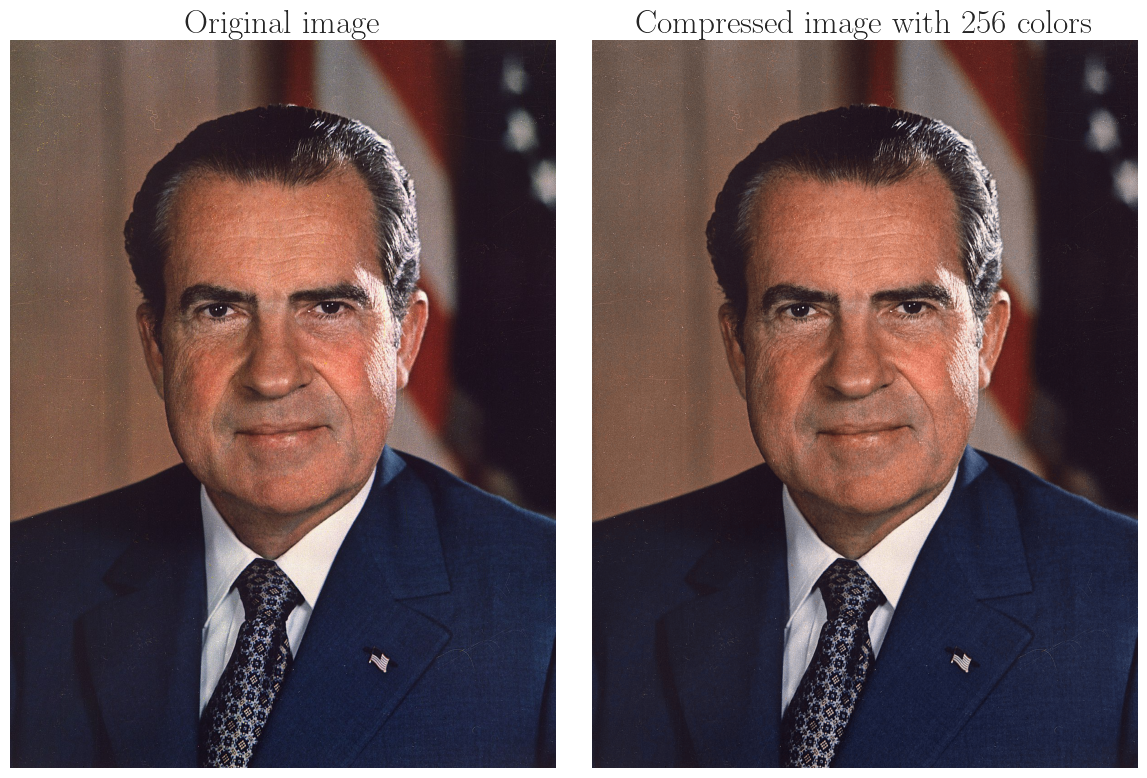
\includegraphics[width=0.5\textwidth]{nixon_compressed.png}
 \caption{A comparison of President Nixon before and after undergoing compression \cite{nixon}}
 \end{figure}

\textbf{Compression Ratio:} Running $k$-means on an image replaces the 3-vector of each pixel with a single element corresponding to the index of the color representative to which the pixel was assigned. In addition, we have a $3\times k$ array that stores the color representatives. When considering images with millions of pixels this added cost becomes trivial. A beneficial consequence of this is that the compression ratio of the algorithm is nearly constant for any choice of $k$ colors less than or equal to 256, as all integers in such a range can be stored using 8-bit unsigned integers (typically the same data type as the original RGB array). This yields a compression ratio of 3, a moderate number in comparison to other compression algorithms like JPEG.  A unique benefit of $k$-means,however, is that the compression ratio is known ahead of time, as each 3-vector will be compressed to a 1-vector regardless of the chosen number of colors.\\

\textbf{Parallelizability}: While the storage cost of $k$-means is held nearly constant for $k\in\{1,\ldots,256\}$, the computational cost of performing the compression quickly becomes quite large when dealing with images of millions of pixels. Thankfully $k$-means is at least partially parallelizable at all steps of the algorithm. Summation can be easily split into chunks with no added memory cost, and minimization can be split on a per-cluster basis. Pooling the minimization task, however, does require passing a copy of all representative vectors to each processor, which could add up to a meaningful amount of memory overhead for large values of $k$.
\end{section}
\begin{thebibliography}{3}
\bibitem{bonald}
Thomas Bonald (2019) \emph{Expectation-Maximization for the Gaussian Mixture Model}, Institut Polytechnique de Paris, https://perso.telecom-paristech.fr/bonald/documents/gmm.pdf.
\bibitem{linalg}
Stephen Boyd and Lieven Vandenberghe (2018) \emph{Introduction to Applied Linear Algebra}, Cambridge University Press.
\bibitem{nixon}
The White House (2022) \emph{Richard M. Nixon}, https://www.whitehouse.gov/about-the-white-house/presidents/richard-m-nixon/, Accessed: 2024-05-18.
\end{thebibliography}
\end{document}